\documentclass[12pt,letterpaper]{article}


\usepackage{amsmath}
\usepackage{amsfonts}
\usepackage{amsthm}
\usepackage{amssymb}
\usepackage{ulem}
\usepackage{tikz}
\usepackage{pgfplots}
\pgfplotsset{compat=1.8}


\newcommand\mybox[2][]{\tikz[overlay]\node[fill=yellow!20,draw=black,inner sep=2pt, anchor=text, rectangle, rounded corners=1mm,#1] {#2};\phantom{#2}}
\usepackage{graphicx}

\newcommand{\Lim}[1]{\raisebox{0.5ex}{\scalebox{0.8}{$\displaystyle \lim_{#1}\;$}}}


\title{Mandatory Assignment 2 of 2}
\author{Håkon Berggren Olsen\\
  \small{MAT2400 - Real Analysis}\\
  \small{University of Oslo}\\
  \small{hakonberggren@gmail.com}
}
\date{Spring 2022}

\begin{document}
\maketitle
\newpage 
 
\section*{Problem 1}
 
Let $f:[-\pi,\pi] \to \mathbb{R}$ be given by $f(x) = |x|$.\\
a) Show that the real Fourier series of $f$ is 
\begin{align}
	\frac{\pi}{2} -\frac{4}{\pi}\sum_{n=0}^\infty \frac{\cos \left[(2n+1)x\right]}{(2n+1)^2}
\end{align}

\noindent\fbox{
    \parbox{\textwidth}{
 	\noindent \\
	As $f(x)=f(-x)$ (even), we have $b_n=0$. For we $a_0$ calculate the average of the function on the inteval $[-\pi, \pi]$
	\begin{align*}
		a_o = \frac{1}{2\pi}\int_0^\pi |x| dx = \frac{\pi}{2}
	\end{align*}
	For the $a_n$ terms we calculate
	\begin{align*}
		a_n &= \frac{1}{\pi}\int_{-\pi}^{\pi} f(x) \cos(nx) dx =  \frac{2}{\pi}\int_{0}^{\pi} x \cos(nx) dx \\
		%a_n &= \frac{2}{\pi}\left[\frac{x \sin(nx)}{n}|_o^\pi - \int_0^\pi \frac{\sin(nx)}{n} dx\right] \\
		a_n &= \frac{2}{\pi}\left[ \frac{\pi \sin(n \pi)}{n}+\frac{\cos(n\pi)}{n^2} -\frac{1}{n^2} \right] \\
		a_n &= \frac{2}{\pi}\left[\frac{\cos(n\pi)}{n^2}-\frac{1}{n^2}\right] \quad ;\quad (\sin(n\pi)=0, \ \forall n \in \mathbb{N})
	\end{align*}
	When $n$ is even $\cos(n\pi) = 1$ and when $n$ is odd $\cos(n\pi)=-1$. Thus
	\begin{align*}
		a_n &= \frac{2}{\pi}\left[\frac{(-1)^n}{n^2}-\frac{1}{n^2}\right]
	\end{align*}

	% Maybe omit this calculation as it is fairly obivous from the equation above?
	%For the terms where $n$ is even, we can substitute with $n=2r$ for $r\in\mathbb{N}$
	%\begin{align*}
	%	a_{2k} &= \frac{2}{\pi}\left[\frac{(-1)^{2k}}{(2k)^2}-\frac{1}{(2k)^2}\right] = \frac{2}{\pi}\left[\frac{1}{(2k)^2}-\frac{1}{(2k)^2}\right] = 0
	%\end{align*}
	We can see that for even $n=2k$ we get $a_{2k}=0$. For odd $n=2k+1$ we have
	\begin{align*}
		a_{2k+1} &= \frac{2}{\pi}\left[\frac{(-1)^{2k+1}}{(2k+1)^2}-\frac{1}{(2k+1)^2}\right]  =  -\frac{4}{\pi}\frac{1}{(2k+1)^2}
	\end{align*}
	Combining 
	\begin{align*}
		|x| = \frac{\pi}{2} -\frac{4}{\pi}\sum_{n=0}^\infty  \frac{\cos \left[(2n+1)x\right]}{(2n+1)^2}
	\end{align*}
    }
}
b) We shall later prove a theorem (Theorem 10.6.2) which implies that 
	\begin{align*}
		f(x) = \frac{\pi}{2} -\frac{4}{\pi}\sum_{n=0}^\infty  \frac{\cos \left[(2n+1)x\right]}{(2n+1)^2}
	\end{align*}
for all $x\in[-\pi,\pi]$. Use this to find the sum of the series $1+\frac{1}{3^2}+\frac{1}{5^2}+\cdot \cdot \cdot \frac{1}{(2n+1)^2}+ \cdot \cdot \cdot$.

\noindent\fbox{
    \parbox{\textwidth}{
 	\noindent \\
	Evaluting the taylor series of $f(x)=|x|$ at $x=0$
	\begin{align*}
		f(0) = 0 = \frac{\pi}{2} -\frac{4}{\pi}\sum_{n=0}^\infty  \frac{1}{(2n+1)^2}
	\end{align*}
	Rearranging
	\begin{align*}
		\sum_{n=0}^\infty  \frac{1}{(2n+1)^2} = \frac{\pi^2}{8} 
	\end{align*}
    }
}
\newline
\noindent
c) Make plots of the finite approximnations 

for $N = 0,1,2$ and compare them to $f$.



\noindent\fbox{
    \parbox{\textwidth}{
 	\noindent \\
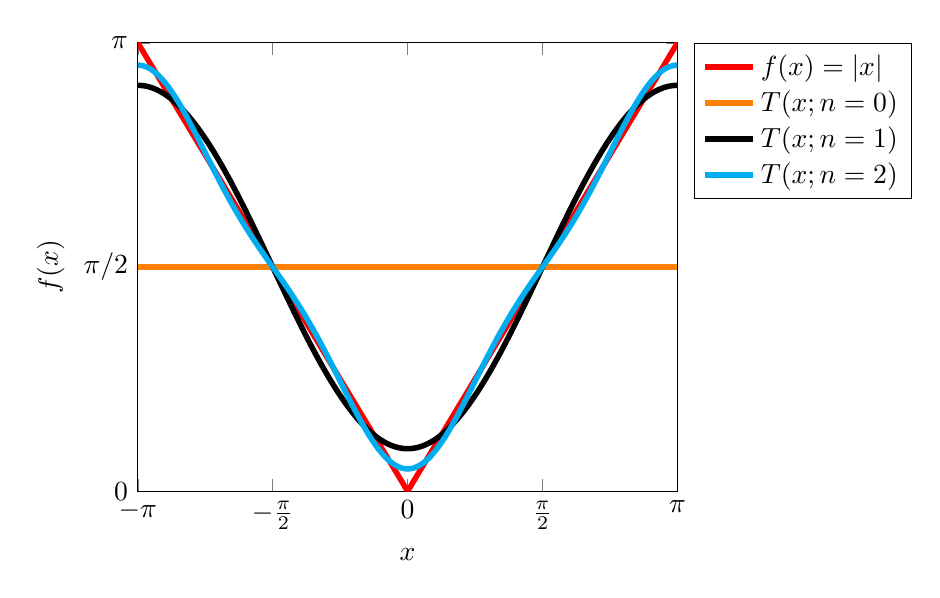
\begin{tikzpicture}
	\centering
	\begin{axis}[
		xmin=-pi,
		xmax=pi,
		ymin=0,
		ymax = pi,
		xtick = {-pi,-pi/2, 0, pi/2, pi},
		xticklabels = {$-\pi$, $-\frac{\pi}{2}$, $0$, $\frac{\pi}{2}$, $\pi$},
		ytick = {0, pi/2, pi},
		yticklabels = {$0$, $\pi/2$, $\pi$},
		xlabel = $x$,
		ylabel = $f(x)$,
        		legend pos=outer north east,
		legend cell align = left,
		smooth,
]
	\addplot[domain=-pi:pi, smooth, samples=200, line width = 2pt, red] {abs(x)};
	\addplot[domain=-pi:pi, smooth, samples=200, line width = 2pt, orange] {pi/2};
	\addplot[domain=-pi:pi, smooth, samples=200, line width = 2pt, black] {pi/2-(4/pi)*(cos(180*x/pi))};
	\addplot[domain=-pi:pi, smooth, samples=200, line width = 2pt, cyan] {pi/2-(4/pi)*(cos(180*x/pi)+cos(3*x*180/pi)/9)};
	\addlegendentry{$f(x)=|x|$}
	\addlegendentry{$T(x;n=0)$}
	\addlegendentry{$T(x;n=1)$}
	\addlegendentry{$T(x;n=2)$}


	\end{axis}
\end{tikzpicture}
    }
}

\newpage
\section*{Problem 2}

Assume that $\{ \bf{e}_n \}_{n\in\mathbb{N}}$ is an orthonormal set in an inner product space $(V, \langle\cdot,\cdot\rangle)$.

a) Show that if $n\neq m$, then $||\bf{e}_n-\bf{e}_m|| = \sqrt{2}$.


\noindent\fbox{
    \parbox{\textwidth}{
 	\noindent \\
	We have the inner product given as 
	\begin{align*}
		||\bf{e}_n-\bf{e}_m||  &= \sqrt{\langle \bf{e}_n -\bf{e}_m,\bf{e}_n -\bf{e}_m \rangle} \\
	\end{align*}
	Using the distributive property of $\langle \bf{u} + \bf{v} , \bf{w} \rangle = \langle \bf{u} , \bf{w} \rangle + \langle  + \bf{v} , \bf{w} \rangle$ :
	\begin{align*}
		&= \sqrt{\langle \bf{e}_n, \bf{e}_n \rangle - 2 \langle \bf{e}_n, \bf{e}_m \rangle + \langle \bf{e}_m, \bf{e}_m \rangle } \\
		&= \sqrt{1^2-2\cdot 0 + 1^2 } = \sqrt{2} \\
	\end{align*}
	where $\langle \bf{e}_n , \bf{e}_m \rangle = 0$ for $m\neq n$. 
	
    }
}
\\
\\
b) Let
\begin{align*}
	S = \{\bf{v} \in V : ||\bf{v} = 1 \}
\end{align*}
be the unit sphere in $V$. Show that $S$ is not compact.


\noindent\fbox{
    \parbox{\textwidth}{
 	\noindent \\
	
	 https://wiki.math.ntnu.no/linearmethods/basicspaces/ballsandspheres
	
	
    }
}

\newpage
\section*{Problem 3}
Recall the Gram-Schmidt process from linear algebra: If $\{ \bf{v}_n\}_{n=0}^\infty$ is a linearly independent sequence in an inner product space $(V, \langle\cdot,\cdot\rangle)$, define a new sequence $\{\bf{u}\}_{n\in\mathbb{N}}$ by
\\

\noindent
Then the new sequence is orthogonal (i.e. $\langle \bf{u}_i, \bf{u}_j \rangle = 0$ for $i \neq j$) and $\text{Span}(\bf{u}_0,\bf{u}_1,...,\bf{u}_n) = \text{Span}(\bf{v}_0,\bf{v}_1,...,\bf{v}_n) $ for all $n$. We get an orthonormal sequence $\{\bf{e}_n\}$ by putting $\bf{e}_n = \frac{\bf{u}_n}{||\bf{u}_n||}$.


a) Let $V = C([0,1], \mathbb{R})$ and define an inner product on $V$ by

\begin{align*}
	\langle u, v \rangle = \int_0^1 u(x)v(x)dx
\end{align*}
Assume that we perform the Gram-Schmidt process on the polynomials $v_0(x)=1, v_1(x)=x, v_2(x)=x^2, ..., v_n(x) = x^n, ...$ and get an orthonormal sequence $e_o(x), e_1(x), e_2(x), ..., e_n(x),...$ Find $e_0(x)$ and $e_1(x)$.


\noindent\fbox{
    \parbox{\textwidth}{
 	\noindent \\
	To find $e_0(x), e_1(x)$ we have
	\begin{align*}
		e_0(x) &= v_0(x) = 1\\
		e_1(x)&= v_1(x) - \frac{\langle v_0(x), v_1(x) \rangle}{\langle v_0(x), v_0(x) \rangle} v_0(x)
	\end{align*}
	Calculating the inner products
	\begin{align*}
		\langle v_0(x), v_1(x) \rangle &= \int_0^1 1 \cdot x dx = \frac{1}{2} \\
		\langle v_0(x), v_0(x) \rangle &= \int_0^1 1 \cdot 1 dx = 1
	\end{align*}

	Dividng by the absolute value we get the orthonormal series. Absolute value of $e_1(x)$ is
	\begin{align*}
		||e_1(x)||^2 &= \langle e_1(x), e_1(x) \rangle\\
		  	      &= \int_0^1 (x-\frac{1}{2})^2 dx = \int_{-\frac{1}{2}}^{\frac{1}{2}} u^2 du\\
			&= \frac{1}{3} \left[ \left( \frac{1}{2}\right)^3-\left( -\frac{1}{2}\right)^3\right]\\
			&= \frac{1}{12}
	\end{align*}	
	And then we get the new, orthogonal vectors
	\begin{align*}
		e_0(x) &= 1 \\
		e_1(x) &= \frac{x}{2\sqrt{3}}-\frac{1}{4\sqrt{3}}
	\end{align*}
    }
}


b) Let $h\in V$ and assume that $\langle h, e_n \rangle = 0$ for $n=0,1,2,...$. Show that $\langle h, p \rangle = 0$ for all polynomials $p$.

\noindent\fbox{
    \parbox{\textwidth}{
 	\noindent \\
	Note: $h$ is "orthogonal" to every orthogonal vector. Therefore it must be orthogonal to every polynomial: Write this arguemnt but in "math".
	https://math.stackexchange.com/questions/400331/show-that-a-vector-that-is-orthogonal-to-every-other-vector-is-the-zero-vector
    }
}



c) Show that $\langle h,h \rangle = 0$, and conclude that $h=0$.
\\
\noindent\fbox{
    \parbox{\textwidth}{
 	\noindent \\
	
		
    }
}

d) Let $f\in V$ and put $\alpha_n = \langle f, e_n \rangle$. Assume that $g(x) = \sum_{n=0}^\infty \alpha_n e_n(x)$ is continous (the sum here is with respect to the norm $|| \cdot ||$ generated by $\langle \cdot, \cdot \rangle$, hence $\lim_{N\to\infty} ||g(x)-\sum_{n=0}^\infty \alpha_n e_n(x)|| = 0$). Show that $g=f$.










\end{document}